\documentclass{beamer}
\usetheme{Malmoe}
\usecolortheme{dove}
%\setbeamertemplate{navigation symbols}{}  %remove navigation symbols
%Deutsch
\usepackage[ngerman]{babel}
\usepackage[utf8]{inputenc}
%Mathe
\usepackage{amsmath}
%Einheiten
\usepackage{siunitx}
%Baumstrukturen
\usepackage{tikz}
\usepackage{tikz-qtree}
\usepackage{textcomp}   % allows \textrightarrow
%Bildquellen
\usepackage{varwidth}
\usepackage{graphicx}
\usepackage{hyperref}

\author{Florian Seligmann}
\title{Die Baupolitik des Augustus}
\date{\textbf{11.6.2018}}

\tikzset{
  invisible/.style={opacity=0},
  visible on/.style={alt={#1{}{invisible}}},
  alt/.code args={<#1>#2#3}{%
    \alt<#1>{\pgfkeysalso{#2}}{\pgfkeysalso{#3}}
  }
}

%Item mit Pfeil
\newcommand{\aitem}{%
\item[$\rightarrow$]
}

%Bildquellen
\newcommand*{\quelle}{%
  \tiny Quelle:
}

%Bilder
\newcommand{\bild}[3]{%
	\begin{figure}
	\centering
  \begin{varwidth}{\linewidth}
    \raggedleft
    \includegraphics[scale=#2, width=\textwidth]{#1}\\
    \quelle{\url{#3}}
  \end{varwidth}
\end{figure}
}

%Einheiten
\sisetup{
  locale = DE ,
  per-mode = symbol
}

%=====================================================================================================================================
\begin{document}

\frame{\titlepage}
\frame{\frametitle{Gliederung}
\tableofcontents
} %End of frame
%-------------------------------------------------------------------------------------------------------------------------------------

%----------------------------------------------Res gestae---------------------------

\frame{\frametitle{Primärquelle - Re gestae}  % http://www.latein-imperium.de/include.php?path=content&mode=print&contentid=126
	\begin{itemize}
		\item Wichtigste Primärquelle: \glqq{}Res gestae Divi Augusti\grqq{}  % Taten des göttliche Augustus
		\item Verfasst mit 76 von Augustus
		\item Aufgestellt im ganzen Reich
		\item Ziel: Macht nicht selbst erstrebt, immer vom Senat \& Volk freiwillig übertragen
	\end{itemize}
}%eof

%----------------------------------------------------------------------------------

\section{Entwicklung der Baupolitik}

\subsection{Zeit der Bürgerkriege}

\frame{\frametitle{Bürgerkriege}
	\begin{itemize}
		\item 44 v. Chr. - 31 v. Chr.
		\pause
		\item Antonius von Ägypten aus
		\aitem Betonung Roms
		\pause
		\aitem Repräsentative Bauten in Rom
		\aitem Caesarkult
	\end{itemize}
}%eof

\frame{\frametitle{Beispiele zur Zeit der Bürgerkriege}
	%Mausoleum Augustus auf Marsfeld
	\begin{center}
		\bild{images/mausoleum_beschnitten.png}{0.5}{http://www.roma-antiqua.de/abbildungen/antikes_rom/marsfeld/2000_351.jpg}
		%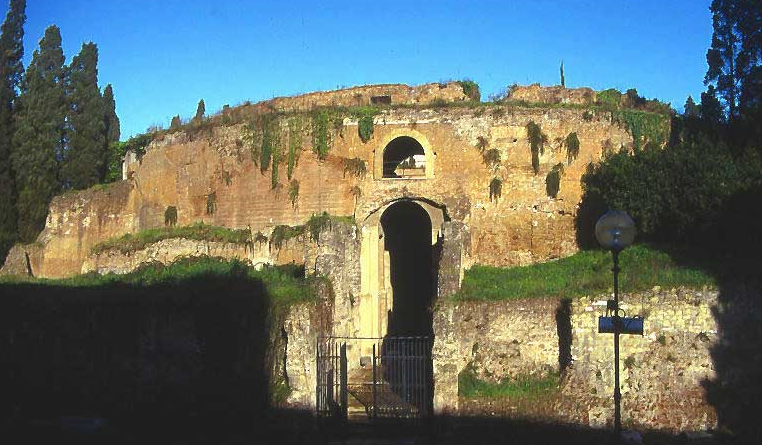
\includegraphics[0.5]{images/mausoleum_beschnitten.png}
	\end{center}
	
}%eof

\frame{\frametitle{Beispiele zur Zeit der Bürgerkriege}
	%Mausoleum Augustus auf Marsfeld
	\bild{images/mausoleum_oben.png}{1.0}{https://www.realmofhistory.com/wp-content/uploads/2017/05/restoration-mausoleum-of-augustus-rome_3-770x437.jpg}
}%eof

\frame{\frametitle{Bürgerkriege}
	\begin{itemize}
		\item Bezug zu Apollo
		\pause
		\item Betonung der Ahnenreihe
		\pause
		\item Über Venus, Aeneas, Iulus Ascanius und Caesar
		\aitem Curia Iulia, Tempel des Divus Iulius auf dem Forum Romanum %Curia Iulia: Senatsgebäude, von Caesar begonnen; Divus Iulius: Tempel für vergöttlichten Caesar -> Lage am Forum Romanum
		\pause
		\item Bezug zu Romulus \textbf{$\rightarrow$} \glqq{}Neubgründer\grqq{}
		\aitem Wohnhaus auf dem Palatin bei der Hütte des Romulus
	\end{itemize}
}%eof

\subsection{Zeit des Prinzipats}

\frame{\frametitle{Prinzipat}
	\begin{quote}
		Da die Stadt nicht so prunkvoll aussah, wie es die Bedeutung des Imperiums verlangte, auch immer wieder von Überflutungen und 				Feuersbrünsten bedroht wurde, verschönerte er sie so, dass er danach mit Recht behaupten konnte, er habe ein Rom aus Ziegeln vorgefunden und eines aus Marmor hinterlassen.
	\end{quote}
	\tiny{Suet. Aug. 28, 3}	%Kaiserbiographien
}%eof

\frame{\frametitle{Prinzipat}
	\begin{itemize}
		\pause
		\item Erneuerung der Infrastruktur %-> Agrippa; "Cloaca Maxima"; Aquaedukte; Straßen; Brandschutz
		\pause
		\item Erneuerung der Tempel %-> Rückkehr zu den Göttern, vor allem Iupiter, Mars, Apollo
		\pause
		\item Fertigstellung vieler Bauwerke
		\pause
		\item Siegesdenkmäler
	\end{itemize}
}%eof

\frame{\frametitle{Marmor}
	\begin{itemize}
		\item Marmor während Republik kaum verwendet
		\item Marmor Symbol für \glqq{}Goldenes Zeitalter\grqq{}.
		\item Kontrolle der Seewege $\rightarrow$ Marmor aus dem ganzen Reich % Machtrepräsentation
		\item Marmor sehr teuer $\rightarrow$ Gebäude oft nur mit Marmor verkleidet
		\item 
	\end{itemize}
}%eof

\section{Ara Pacis}

\frame{\frametitle{Ara Pacis}
	\bild{images/ap_totale.png}{0.35}{https://www.bluffton.edu/homepages/facstaff/sullivanm/italy/rome/arapacis/0081.jpg}
}%eof


\frame{\frametitle{Ara Pacis Augustae - Eckdaten}
	\begin{itemize}
		\item 13 v. Chr. vom Senat in Auftrag gegeben
		\item Geweiht am 30. Januar 9 v. Chr. (Geburtstag der Livia)
		\pause
		\item 11.63m x 10.62m
		\pause
		\item Aufbau ähnlich einem \glqq{}templum minus\grqq{} %früher Holzzaun um Altar in der Mitte
		\aitem Aber aus massivem lunensischem Marmor % Carrara-Marmor, wg. Provin Luna
	\end{itemize}
} %eof

\frame{\frametitle{Fundgeschichte}
	\begin{itemize}
		\item Unter Tiberschlamm begraben
		\pause
		\item 1568 Erste Entdeckungen
		\item 1879 Indentifikation als Ara Pacis
		\pause
		\item Ausgrabungen 1903 \& 1937/38 %Mussolini -> Identifikation mit Augustus
		\item Heute Rekonstruktion
	\end{itemize}
}%eof

\frame{\frametitle{Aufgaben}
	\begin{itemize}
		\item Rückblick auf Griechenland \& die Republik
		\item Versprechen eines \glqq{}Goldenen Zeitalters\grqq{} 
	\end{itemize}
}%eof

\frame{\frametitle{Gestaltung}
	\begin{itemize}
		\item Interpretation sehr umstritten
		\item Einteilung %Oben Szenen, Handlungen; unten Natur, Wildheit, Roheit /Blütezeit
	\end{itemize}
}%eof
%--------------------------------------------horologium-----------------
\frame{\frametitle{Horologium solarium Augusti}
	\bild{images/horologium.png}{0.1}{http://cdn.ipernity.com/134/84/75/24228475.ef26a17d.640.jpg?r2}
}%eof
\frame{\frametitle{Horologium solarium Augusti}
	
}%eof

\end{document}